\chapter{Writing down nature: derivatives}
\label{sec:derivatives}

\section{Invitation to calculus from a physicist}

\prerequisites{graphs, functions, kinematic variables}

\subsection{The mission of calculus}

Calculus is in two parts: differential and integral, which is linked by the fundamental theorem of calculus. Calculus \emph{links} physical systems to mathematical equations, so we can \emph{predict} the future of a system from the solution of those equations. But before we \emph{predict}, we must describe the system first: we must find a \emph{link}. And that's what we're going to do in this chapter.

The system that we'll use in this chapter is a mass that's traveling with some speed. We'll see how the attempt to describe this system naturally give birth to \emph{derivatives}. In the next chapter, we'll find the solution to the equation we've written. And at the end, we'll develop an intuition that
\begin{enumerate}[noitemsep]
    \item Derivatives measures the rate of change of a function w.r.t. a variable.
    \item Derivatives can be thought of the slope of a graph
    \item The universe is described in the language of differential equations
\end{enumerate}

\subsection{The notation of derivative calculus}
\label{sec:notation_of_calculus_derivative}

If $a$ is a variable, then $\odif{a}$ is a very small quantity of $a$ a.k.a. an \textbf{infinitesimal}. E.g., if $\vv{x}$ is displacement, then $\odif{\vv{x}}$ is a very small displacement. If $t$ is the time, then $\odif{t}$, a very short time.

We can also find ratio between infinitesimal. E.g., the ratio between some small distance and some short time, $\odv{\vv{x}}{t}$, we get the speed $\vv{v}$.

\subsection{Message from a physicist about the pedagogy}

Physics is about trying to understand how nature works. What we do in physics is that we first describe a system using mathematical equations, then use the solution of that equation to reveal the nature of that system. Here, I'd do the same.

If I were teaching a class, I'd tell you about car design. But, this is a textbook, and trying to deliver the same story here isn't that concise and cohesive. So, instead of following a story about cars, I'd like you to hop on with me and analyze the mechanics of a \textbf{speedometer}, which I reckon is the best introduction to calculus there is.

\section{Speed and instantaneous rate of change}
\label{sec:speedandinstantaneousrateofchange}

Let's analyze how a car \textbf{speedometer} work. If we're traveling at a speed $\qty{5}{\meter\per\second}$, when \emph{exactly} are we traveling at $\qty{5}{\meter\per\second}$? You could say $\vv{v} = \qty{5}{\meter}$ \emph{at the moment of measurement}. That's like saying, ``Oh, I can find the speed of the car by just taking a picture of it.'' But that's illegal! To calculate speed, we have to compare two points in space through time. Or, the rate of change of distance through time:
\begin{equation}
    \vv{v} = \frac{\vv{s}_2 - \vv{s}_1}{t_2 - t_1}. \label{eq:averagevelocity}
\end{equation}
While it may seem like cameras grab snapshots in an instant, they actually need time to take in light to construct an image, they need some \emph{exposure time} $\Dd{t}$.

To get a ``not blurred image'' of a moving object, we reduce the exposure time. If the exposure time is too long, the object will be smeared out. This effect is known as motion blur, which is normally undesired. But motion blur actually helps out a lot with measuring velocity. In which the velocity is just 
\begin{equation}
    \vv{v} = \frac{\textrm{Distance between the smear and the main object}}{\textrm{Exposure time}}.
\end{equation}
As illustrated in \cref{fig:car-motion-blur}, the motion blur clearly shows us the change in position of the car over the exposure time.
\begin{figure}[ht]
   \centering
   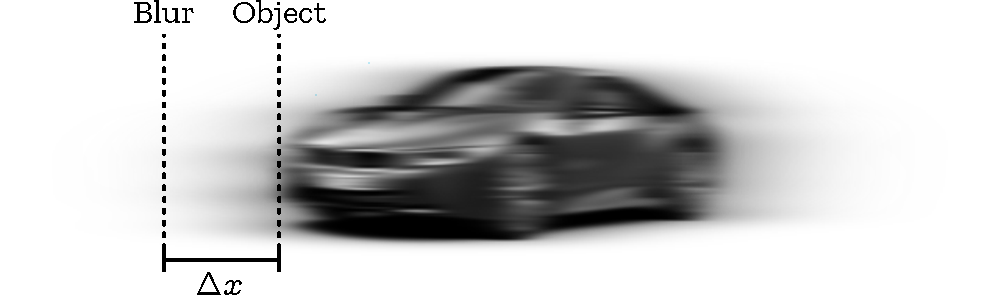
\includegraphics[width = \textwidth]{derivatives/motionblurredcar.pdf} 
   \caption{Calculating the velocity of a car from motion blur.}
   \label{fig:car-motion-blur}
\end{figure}

But what will happen with shorter exposure time? Does the motion blur disappear? No! The blur is still there, but it's just smaller. Typically, $\qty{12}{\ms}$ exposure time is short enough to create a ``focused image''. But it's just an illusion that came from the limitation of the screen's ability to reproduce such little blur. If our camera and screen is good enough, we can \emph{always} calculate the velocity of the car from the blur. The smaller the exposure time, the more detailed the image is, and the closer you'll get to the exact $\vv{v}$ at that moment in time. Finally, if we let the exposure time become infinitesimally short, we can say the $\vv{v}$ we got is \emph{the velocity at that exact point}. Or as we call it, the \textbf{instantaneous velocity}. By using the said calculus notation in \cref{sec:notation_of_calculus_derivative}, we can just write this as
\begin{equation}
    \vv{v} = \odv{\vv{x}}{t}, \label{eq:first_intro_to_derivative}
\end{equation}
and here it is ladies and gentlemen, the \textbf{derivative}: the measure of rate of change.

From here on out, I shall use \emph{derivative} and \emph{rate of change} interchangeably. So, every time you see \emph{derivative}, think \emph{rate of change}.

\section{An attempt to define derivatives}

Mathematically, a \textbf{derivative} is a measure of a function's rate of change with respect to a variable. In the previous example, $\vv{x}$ is a function that's dependent on time, and its derivative w.r.t. time, $\vv{v}$, is measuring the rate of change of function $\vv{x}(t)$ through time $\odif{t}$.

To find an explicit expression for derivative, let's say we have two points in spacetime $(\vv{x}_1, t_1)$ and $(\vv{x}_2, t_2)$. The change in $\vv{x}$ is $\vv{x}_2 - \vv{x}_1$, and the change in time is $t_2 - t_1$. The derivative of position w.r.t. time is then just
\begin{equation}
    \vv{v} = \odv{\vv{x}}{t} = \frac{\vv{x}_2 - \vv{x}_1}{t_2 - t_1}. \label{eq:derivative1}
\end{equation}
Let $t_2 = t + h$. Then, $\vv{x}_2 = \vv{x}(t + h)$ and $\vv{x}_1 = \vv{x}(t)$. The time difference used to calculate $\vv{v}$ must be miniscule: infinitesimally small. I have to introduce the notion of limits, which is just a fancier way of saying ``very close to, but not''
\begin{align}
    \vv{v} = \odv{\vv{x}}{t} &= \lim_{h \appr 0}\frac{\vv{x}(t + h) - \vv{x}(t)}{(t + h) - t} \\
    \vv{v} = \odv{\vv{x}}{t} &= \lim_{h \appr 0}\frac{\vv{x}(t + h) - \vv{x}(t)}{h}.
\end{align}
The equation above is what we generally refer to as the \emph{definition of derivative}. Then, we just extend this relation to any function $f(x)$, which requires just a substitution of variables. And then we get:
\begin{df}{Naive definition of derivative}{derivative_naive}
    \index{derivatives!naive definition}A derivative of a function $f(x)$ w.r.t. a variable $x$ is the rate of change of $f(x)$ w.r.t. $x$, and it is written as
    \begin{equation}
        \odv{f(x)}{x}~\textrm{or}~\odv{x}(f(x)),
    \end{equation}
    where
    \begin{equation}
        \odv{f(x)}{x} = \lim_{h \appr 0}\frac{f(x + h) - f(x)}{h}.\label{eq:naive_definition_of_derivative}
    \end{equation}
\end{df}
\Cref{eq:naive_definition_of_derivative} directly reads:
\begin{quote}
    The derivative of $f(x)$ with respect to $x$ is $\frac{f(x + h) - f(x)}{h}$ where $h$ is very close to $0$, but $h$ is strictly not $0$.
\end{quote}

\paragraph{On notation:} So far, we've been using the Leibniz's notation for derivatives, and it has the property that derivatives behave exactly like fractions, and you can cancel terms.
\begin{equation}
    \odv{a}{b}\times\odv{b}{c} = \odv{a}{c}.\label{eq:prechainrule}
\end{equation}
But, this isn't the only accepted notation. Multiple great mathematicians have come up with their own, and some are better than others in certain cases. I'd introduce other notations later on if necessary.

\section{The geometrical interpretation of the derivative}

\begin{wrapfigure}[15]{l}{0.4\textwidth}
    % \centering
    % \begin{subfigure}{0.45\textwidth}
        \centering
        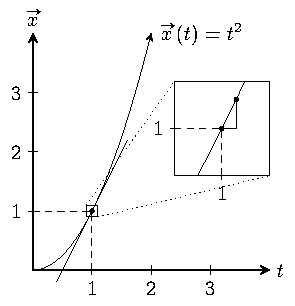
\includegraphics{derivatives/positionversustime}
        \caption{Position vs. time graph where $\protect\vv{x}(t) = t^2$.}
        \label{fig:position_versus_time}
    % \end{subfigure}
    % \begin{subfigure}{0.4\textwidth}
    %     \centering
    %     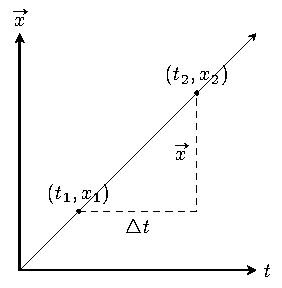
\includegraphics{derivatives/positionversustime2}
    %     \caption{A ball traveling at constant velocity.}
    %     \label{fig:position_versus_time2}
    % \end{subfigure}
    % \caption{Various position versus time graph.}
\end{wrapfigure}

To interpret derivatives, notice that \Cref{eq:derivative1} looks a lot like the slope equation
\begin{equation}
    m = \frac{y_2 - y_1}{x_2 - x_1}. \label{eq:slope_equation}
\end{equation}
We've also seen that \cref{eq:derivative1} is analogous to the definition of derivative \cref{eq:naive_definition_of_derivative}. So is the derivative just the slope of a line? If it is, then what is the $y$-axis and the $x$-axis of a graph?

We can compare \cref{eq:slope_equation} to \cref{eq:derivative1}: the $y$-axis should be the position $\vv{x}$, and the $x$-axis, the time $t$. If we draw that out, we'll get the $x$-$t$ graph, which can encode the exact trajectory of an object. An example of which is shown in \cref{fig:position_versus_time}.

But what does this have to do with derivatives? \Cref{eq:slope_equation} only works for straight line! Well, here's the beauty of it. If you zoom into any points on a curve, eventually, it will look like a line. And thus, \emph{the derivative zooms into the curve at some point, and chooses two very close points on the curve and calculate its slope. In which, that slope represents the rate of change of the function at that point.}

\section{Evaluation of derivatives: method of increments}

Here, I'll give you an example of evaluating the derivative by using the definition, a.k.a. the \textbf{method of increments.}

In \cref{fig:position_versus_time}, the function $\vv{x}(t)$ is just $t^2$: the position at any time $t$ is $t^2$. I'd evaluate the velocity at $t = \qty{1}{\second}$. We start from \cref{eq:naive_definition_of_derivative}:
\begin{align*}
    \vv{v}(1) = \frac{\vv{x_2} - \vv{x_1}}{t_2 - t_1} &= \lim_{h \appr 0}\frac{\vv{x}(1 + h) - \vv{x}(1)}{(1 + h) - 1} \\
    &= \lim_{h \appr 0}\frac{(1 + h)^2 - 1}{h} \\
    &= \lim_{h \appr 0}\frac{2h + h^2}{h} \\
    &= \lim_{h \appr 0}2 + h.
\end{align*}

Since $h$ is very close to zero, we approximate $2 + h$ as $2$. Imagine comparing $2$ to $10^{-10}$. The $10^{-10}$ wouldn't make a noticeable difference, and we can ignore it. Therefore, $\vv{v}(t = \qty{1}{\second}) = \qty{2}{\meter\per\second}$.

Now, try evaluating $\vv{v}(t = \qty{3}{\second})$ for $\vv{x}(t) = t^3$. You should get $\qty{81}{\meter\per\second}$. As a hint, you can also ignore $h^2$ because if $h < 1$, then $h^2 < h$.

\section{Higher order derivatives}

\index{derivatives!higher order}
In kinematics, there are a whole set of quantities that can describe an object's trajectory, e.g., the acceleration, which is defined to be the rate of change of velocity w.r.t. time:
\begin{equation*}
    \vv{a}(t) = \odv{\vv{v}(t)}{t}.
\end{equation*}
\begin{wraptable}[12]{l}{0.35\textwidth}
    \begin{tabular}{c | c}
        Order & Name \\
        \hline
        1 & Velocity/Speed \\
        2 & Acceleration \\
        3 & Jerk \\
        4 & Snap/Jounce \\
        5 & Crackle \\
        6 & Pop
    \end{tabular}
    \caption{Higher order derivatives of position w.r.t. time}
    \label{tab:jerksnapcracklepop}
\end{wraptable}
But the $\vv{v}$ is also the rate of change of position w.r.t. time. Thus,
\begin{equation*}
    \vv{a}(t) = \odv{\vv{v}(t)}{t} = \odv*{\ab(\odv{\vv{r}(t)}{t})}{t} = \odv[ord = 2]{\vv{r}(t)}{t}, 
\end{equation*}
where $\vv{r}$ is any position vector.

The $\odif[ord = 2]{\vv{r}}$ and $\odif{t}^2$ is just a matter of symbolic manipulation and should only be interpreted as just a shorthand. $\vv{a}$ is called the \textbf{second order derivative} of $\vv{r}$ because you've differentiated $\vv{r}$ twice. \textbf{Higher order derivatives} of position w.r.t. time is listed in \cref{tab:jerksnapcracklepop}.

\section{Expressing nature: basic differential equations}
\label{sec:basicdifferentialequations}

\begin{wrapfigure}[14]{r}{0.4\textwidth}
    \centering
    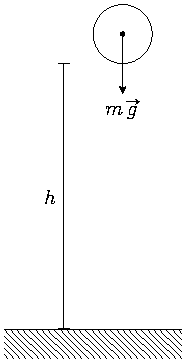
\includegraphics{derivatives/simplemotion}
    \caption{A ball dropped from height $h$}
    \label{fig:ball_dropped_from_a_height}
\end{wrapfigure}
The dynamics of a physical system is universally described by the famous Newton's second law $\vv{F} = m\vv{a}(t)$, which in derivatives form becomes:
\begin{equation}
    \vv{F} = m\odv[ord = 2]{\vv{r}(t)}{t}. \label{eq:newton_second_law}
\end{equation}
Let's try to describe a simple system with this. In \cref{fig:ball_dropped_from_a_height}, a ball is dropped from height $h$. The Earth's gravity pulls the ball with force $mg$ where $m$ is the mass of the ball, and $\vv{g}$, the acceleration from Earth's gravity. Newton's second law tells us that
\begin{align}
    \vv{F} &= m\odv[ord = 2]{\vv{r}(t)}{t} \nonumber\\
    m\vv{g} = m\odv[ord = 2]{\vv{r}(t)}{t} &\quad \textrm{or,} \quad \vv{g} = \odv[ord = 2]{\vv{r}(t)}{t},
\end{align}
which is sometimes called the \textbf{equation of motion}, which packs every information about this system you'd ever want. It directly reads as:
\begin{quotation}
    The acceleration of the ball is equals to $g$.
\end{quotation}
If you've stayed for this long, congratulations! You now have the power to describe every physical systems with mathematical equations using derivatives: the measure of the rate of change. But it might not be as useful as yet, just as a hammer may seem useless if used to paint, derivatives falls apart when you ask about the future of the system. E.g., how long the ball takes to reach the ground? Or, what's the position of the ball at a certain time? That's the job of the integral to solve, and we'll do so in the next chapter.

\conclusion

\begin{enumerate}[noitemsep]
    \item The concept of approaching can be used to bypass dividing by zero.
    \item Derivatives are rate of change of a function w.r.t. a variable which can be evaluated by the method of increments.
    \item Derivatives can be thought as the slope of a graph, or the tangent to a curve.
    \item Physical systems can be described by differential equations of different forms. One of them is the Newton's formulation stated in \cref{eq:newton_second_law}
\end{enumerate}

\begin{remark}{}{derivatives}
    \begin{enumerate}
        \item In \cref{sec:speedandinstantaneousrateofchange}, we zoomed in on the graph to approximate the function as a line. Actually, this is quite literally the whole idea of derivatives. If we dig in further in calculus, sometimes the rate of change analogy doesn't even make sense. However, saying that the derivative tries to approximate every function as a line works in all scenario. Though, it's quite abstracted away from the world.
    \end{enumerate}
\end{remark}